\textbf{COLUNI 2020 -- Questão 23}\par\medskip Já se passaram 100 anos desde a observação de um eclipse solar que permitiu a comprovação da teoria da relatividade geral formulada por Einstein. Essa observação foi realizada em 1919, na cidade nordestina de Sobral e, simultaneamente, no país São Tomé e Príncipe.

\par

De acordo com essa teoria, a luz proveniente das estrelas é desviada ao passar próxima ao Sol, como ilustra a figura abaixo. O eclipse permitiu a observação desse fenômeno, pois, durante o dia, a Lua encobriu a luz solar para observadores situados na umbra, região escura do eclipse.

\par

Estrela 1 Luz da Estrela 1

\par

TERRA                 LUA                                               SOL

\par

Luz da Estrela 2 Estrela 2

\par

Dos objetos listados abaixo, aquele que provoca um desvio na luz que incide sobre ele, semelhante ao que ocorre na figura acima, é:

% COLUNI-AUTO-FIGURES-BEGIN
\begin{figure}[htbp]
\centering
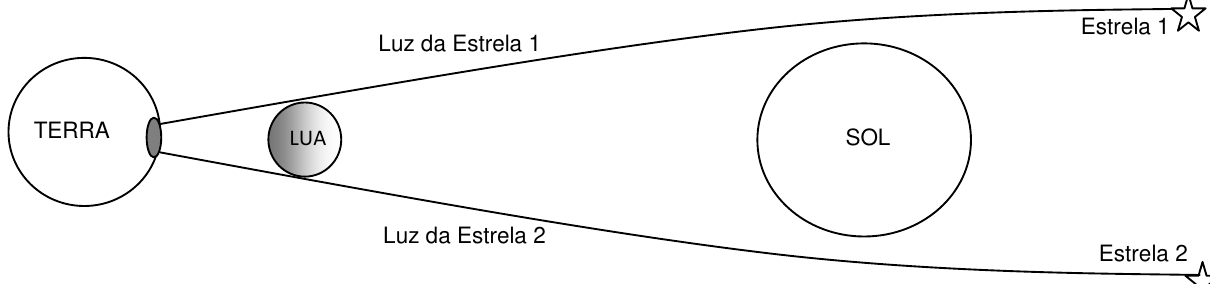
\includegraphics[width=0.95\linewidth]{static/simulados/coluni/figuras/2020/questao-23/figura-1.png}
\end{figure}
% COLUNI-AUTO-FIGURES-END
\begin{enumerate}
\item um espelho plano.
\item um espelho convexo.
\item uma lente divergente.
\item uma lente convergente.\end{enumerate}
